\documentclass[bj, preprint]{imsart}
\RequirePackage[OT1]{fontenc}
\RequirePackage[colorlinks,citecolor=blue,urlcolor=blue]{hyperref}
\usepackage{amsthm,amsmath,natbib,booktabs,cleveref}
\newcommand{\cexp}[1]{\left<#1\right>}
\usepackage{bbm}
\newcommand{\onebb}{\mathbbm{1}}
\newcommand{\Ebb}{\mathbb{E}}

% put your definitions there:
\endlocaldefs
\usepackage{float}
\usepackage[]{graphicx}
\graphicspath{ {fig/} }
\usepackage{enumitem}
\usepackage{xcolor}
\usepackage[colorinlistoftodos,prependcaption]{todonotes}
\usepackage[group-separator={,}]{siunitx}

\newcommand{\dat}[1]{\todo[color=green!40]{[Dat]#1}}
\newcommand{\simon}[1]{\todo[color=blue!40]{[Simon]#1}}

\startlocaldefs
\numberwithin{equation}{section}
\theoremstyle{plain}
\newtheorem{thm}{Theorem}[section]
\newtheorem{lem}{Lemma}[section]
\newtheorem{cor}{Corollary}[section]
\newtheorem{prop}{Proposition}[section]
\theoremstyle{remark}
\newtheorem{rem}{Remark}[section]

% -----------------------------------------------------------------------------
% algorithms
\usepackage[]{algorithmicx}
\usepackage[]{algorithm}
\usepackage{algpseudocode}
\algnewcommand\algorithmicparameters{\textbf{Parameters:}}
\algnewcommand\PARAMETERS{\item[\algorithmicparameters]}
\renewcommand\algorithmicprocedure{\textbf{Procedure:}}
\algnewcommand\PROCEDURE{\item[\algorithmicprocedure]}
\algnewcommand\algorithmicendprocedure{\textbf{End Procedure}}
\algnewcommand\ENDPROCEDURE{\item[\algorithmicendprocedure]}
\algnewcommand\algorithmicinput{\textbf{Input:}}
\algnewcommand\INITIALIZE{\item[\algorithmicinitialize]}
\algnewcommand\algorithmicinitialize{\textbf{Initialize:}}
\algnewcommand\INPUT{\item[\algorithmicinput]}
\algnewcommand\algorithmicoutput{\textbf{Output:}}
\algnewcommand\OUTPUT{\item[\algorithmicoutput]}
\renewcommand{\algorithmicwhile}{\textbf{While}}
\renewcommand{\algorithmicend}{\textbf{End}}
\renewcommand{\algorithmicif}{\textbf{If}}
\renewcommand{\algorithmicelse}{\textbf{Else}}
\renewcommand{\algorithmicrepeat}{\textbf{Repeat:}}
\renewcommand{\algorithmicuntil}{\textbf{Until}}
\renewcommand{\algorithmicfor}{\textbf{For}}
\renewcommand{\algorithmicdo}{\textbf{do:}}


% -----------------------------------------------------------------------------
% math macros
\usepackage{amsfonts}
\usepackage{amssymb}
\usepackage{amsthm}
\usepackage{bbm}
\usepackage{amsmath}
% general
\DeclareMathOperator{\eps}{\varepsilon}
% dx with spacing
\makeatletter \renewcommand\d[1]{\ensuremath{%
  \,\mathrm{d}#1\@ifnextchar\d{\!}{}}}
\makeatother
% norms
\newcommand{\vertiii}[1]{{\left\vert\kern-0.25ex\left\vert\kern-0.25ex\left\vert #1 
    \right\vert\kern-0.25ex\right\vert\kern-0.25ex\right\vert}}
\newcommand{\vertii}[1]{{\left\vert\kern-0.25ex\left\vert #1 
    \right\vert\kern-0.25ex\right\vert}}
\newcommand{\verti}[1]{{\left\vert #1 
    \right\vert}}
% inner product
\newcommand{\inprod}[1]{{\left\langle #1 
    \right\rangle}}
% text operators
\DeclareMathOperator{\ind}{\mathbbm 1}
\DeclareMathOperator{\ddd}{,\ldots ,}
\DeclareMathOperator{\TV}{TV}
\DeclareMathOperator{\dist}{dist}
\DeclareMathOperator{\diag}{diag}
\DeclareMathOperator{\im}{Im}
\DeclareMathOperator{\iid}{i.i.d.}
\DeclareMathOperator{\MH}{MH}
\DeclareMathOperator{\tr}{tr}
\DeclareMathOperator{\MTM}{MTM}
\DeclareMathOperator{\prox}{\bf prox}
%caligraphic fonts
\DeclareMathOperator{\cA}{\mathcal A}
\DeclareMathOperator{\cB}{\mathcal B}
\DeclareMathOperator{\cC}{\mathcal C}
\DeclareMathOperator{\cD}{\mathcal D}
\DeclareMathOperator{\cF}{\mathcal F}
\DeclareMathOperator{\cG}{\mathcal G}
\DeclareMathOperator{\cH}{\mathcal H}
\DeclareMathOperator{\cI}{\mathcal I}
\DeclareMathOperator{\cK}{\mathcal K}
\DeclareMathOperator{\cL}{\mathcal L}
\DeclareMathOperator{\cN}{\mathcal N}
\DeclareMathOperator{\cO}{\mathcal O}
\DeclareMathOperator{\cP}{\mathcal P}
\DeclareMathOperator{\cQ}{\mathcal Q}
\DeclareMathOperator{\cS}{\mathcal S}
\DeclareMathOperator{\cT}{\mathcal T}
\DeclareMathOperator{\cW}{\mathcal W}
\DeclareMathOperator{\cX}{\mathcal X}
\DeclareMathOperator{\cY}{\mathcal Y}
%bold symbols
\DeclareMathOperator{\b0}{\mathbf 0}
\DeclareMathOperator{\b1}{\mathbf 1}
\DeclareMathOperator{\bX}{\mathbf X}
\DeclareMathOperator{\bx}{\mathbf x}
\DeclareMathOperator{\bB}{\mathbf B}
\DeclareMathOperator{\bD}{\mathbf D}
\DeclareMathOperator{\bR}{\mathbf R}
\DeclareMathOperator{\bbeta}{\boldsymbol \beta}
%tilde and bold symbols
\DeclareMathOperator{\tD}{\tilde{\bD} }
%convergences
\DeclareMathOperator{\convP}{\overset{\bP}{\rightarrow}}
\DeclareMathOperator{\convps}{\overset{p.s.}{\rightarrow}}
\DeclareMathOperator{\convL}{\overset{\mathcal L}{\rightarrow}}
\DeclareMathOperator{\convL2}{\overset{\mathcal L_2}{\rightarrow}}
\DeclareMathOperator{\convD}{\overset{\mathcal D}{\rightarrow}}
%long convergence
\DeclareMathOperator{\lconvP}{\;\overset{\bP}{\longrightarrow}\;}
\DeclareMathOperator{\lconvps}{\;\overset{p.s.}{\longrightarrow}\;}
\DeclareMathOperator{\lconvL}{\;\overset{\mathcal L}{\longrightarrow}\;}
\DeclareMathOperator{\lconvL2}{\;\overset{\mathcal L_2}{\longrightarrow}\;}
\DeclareMathOperator{\lconvD}{\;\overset{\mathcal D}{\longrightarrow}\;}
%operators with indeces underneath
\DeclareMathOperator*{\argmax}{arg\,max}
\DeclareMathOperator*{\argmin}{arg\,min}
%blackbord fonts
\DeclareMathOperator{\bbE}{\mathbb E}
\DeclareMathOperator{\bbN}{\mathbb N}
\DeclareMathOperator{\bbR}{\mathbb R}
\DeclareMathOperator{\bbP}{\mathbb P}
\DeclareMathOperator{\bbZ}{\mathbb Z}
% -----------------------------------------------------------------------------


\begin{document}

\begin{frontmatter}

\title{{\Large STATS 507 Project Preliminary Report:} \\ 
\bf \texttt{MovieLens} Datasets---Predicting and Analyzing User Ratings of Movies}
\runtitle{\texttt{MovieLens}---Predicting and Analyzing Movie Ratings}

\begin{aug}
\author{
\fnms{Trong Dat} 
\snm{Do}
\thanksref{a,e1}
\ead[label=e1,mark]{dodat@umich.edu}
}
\and
\author{
\fnms{Simon} 
\snm{Fontaine}
\thanksref{a,e2}
\ead[label=e2,mark]{simfont@umich.edu}
}
\address[a]{University of Michigan, Department of Statistics. West Hall, 1085 South University, Ann Arbor, MI, U.S.A., 48109. \printead{e1,e2}}
\runauthor{Trong Dat Do and Simon Fontaine}
\affiliation{University of Michigan, Department of Statistics}
\end{aug}



\begin{abstract}
\textbf{Abstract.} The \texttt{MovieLens} datasets contain user ratings of movies as well as movie and user information. In this preliminary report, we consider four predictive models of the ratings based on the available information: $K$-nearest-neighbors, neural networks, matrix completion using singular value decomposition and  restricted Bolztmann machine. We tune all models to finally compare them on their out-of-sample performance. All the code and results can be found at \url{https://github.com/fontaine618/507-Project/}.
\end{abstract}

\end{frontmatter}


\tableofcontents

%------------------------------------------------------------------------------
\section{The \texttt{MovieLens} Datasets}\label{sec:dataset}

The \texttt{MovieLens} datasets \citep{harper2015MovieLensDatasetsHistory} contains user ratings of a variety of movies continuously collected starting from 1998. 
In addition to the \texttt{user}-\texttt{movie}-\texttt{rating} pairings, the datasets contains information about movie genres, word tagging of movies provided by users and user demographic information. 

We will consider the \texttt{MovieLens 100K Dataset}\footnote{Available at \url{https://grouplens.org/datasets/movielens/100k/}}, which is one of the multiple datasets provided by \texttt{GroupLens}\footnote{Organization website: \url{https://grouplens.org/}}. 
We will be interested in this particular dataset because it contains additional demographic information about the users in the dataset. 
To include tagging information, we also consider the \texttt{MovieLens Tag Genome Dataset}\footnote{Available at \url{https://grouplens.org/datasets/movielens/tag-genome/}}. 
Here is a summary of the contents of the datasets that will be used\footnote{From the \texttt{README.txt} file attached to the datasets (\url{http://files.grouplens.org/datasets/movielens/ml-100k-README.txt}, \url{http://files.grouplens.org/datasets/tag-genome/README.html)}}:

\begin{description}
	\item[\texttt{MovieLens 100K Dataset}] 
	The dataset was collected from the \texttt{MovieLens} website (\url{movielens.umn.edu}) between September 19th, 1997 through April 22nd, 1998. 
	It has been pre-processed and cleaned to include only examples where the users have made at least 20 ratings during the collection period and where demographic information are complete. 
	In the \texttt{u.data} file, there are \num{100000} ratings on the scale of 1 to 5, taking only integer values. 
	It contains the following entries: \texttt{user id}, \texttt{item id}, \texttt{rating}, \texttt{timestamp}. 
	In the \texttt{u.item} file, there are \num{1681} movies with the following information: \texttt{movie id}, \texttt{movie title}, \texttt{release date}, \texttt{IMDb URL} and 19 columns indicating movie genre with 0-1 encoding where 1 denotes that the movie is of the corresponding genre. 
	In the \texttt{u.user} file, there are \num{943} users with the following information: \texttt{user id}, \texttt{age}, \texttt{gender}, \texttt{occupation} (see \texttt{u.occupation} file for details) and \texttt{zip code}.
	\item[\texttt{MovieLens Tag Genome Dataset}] 
	This dataset contains tagging information of \num{9734} movies and \num{1128} tags. 
	In particular, the \texttt{tag\_relevance} file contains the relevance of all tags for all movies reported on a continuous scale from 0 to 1, where 1 indicates strong relevance.
\end{description}


%------------------------------------------------------------------------------
\section{Research Questions}\label{sec:questions}

\subsection{Prediction Modeling}

Our first research question is to construct a predictive model for the user ratings using the available information. 
In particular, we wish to produce a model that is able to accurately predict the movie rating (for some movie already in the dataset) by a given user (also in the dataset). 
This model could then be part of a \textit{recommendation system} where the predicted rating could be used as input to produce the recommendations.

\subsection{Exploratory Analysis}

A secondary research question we are interested in is to analyze the effect of the available information on the user ratings. 
For example, we could look for genres and tags that are related to movies with better ratings. 
Then, we can perform more granular analyses using the demographic data: this could allow to extract correlations between population groups and movie interests. 
The insights recovered from such analyses could be relevant for decision-making such as identifying which movies to produce and which population groups to target with advertisement.

%------------------------------------------------------------------------------
\section{Methodology}\label{sec:method}

%------------------------------------------------------------------------------
\subsection{Data Pre-processing}\label{subsec:method.preprocess}

The \texttt{MovieLens 100K Dataset} and the \texttt{MovieLens Tag Genome Dataset} have both been extensively cleaned by \texttt{GroupLens}\footnote{See the two \texttt{README} files for details: \url{http://files.grouplens.org/datasets/movielens/ml-100k-README.txt} and \url{http://files.grouplens.org/datasets/tag-genome/README.html}}. 
Thus, the main pre-processing we have to perform is the merging of the different datasets and the creation of the training and testing sets.

%------------------------------------------------------------------------------
\subsubsection{Merging the Datasets}\label{subsubsec:method.preprocess.merge}

First, the three datasets in \texttt{MovieLens 100K Dataset}, corresponding to user data, movie data and the ratings, have unique IDs which allows us to easily match them. 
There were no ratings which we were unable to match to users and/or movies in these datasets.

Second, the \texttt{MovieLens Tag Genome Dataset} also has unique IDs identifying movies, but they differ from those in the \texttt{MovieLens 100K Dataset}. 
Hence, we resort to matching the movie on the movie name. 
Direct matching of the strings allowed of to match a large proportion ($\sim$80\%) of the movies. 
There were also some movie that we were able to match using simple rules. 
For example, the movie names include the year of publication which were often mismatched by a year and prevented direct matching. 
Also, other movie names included the original name (in a foreign language) in either of the two datasets which prevented direct matching, but could still be detected. 
Finally, visual inspection (mostly by hand) of the remaining unmatched movies allowed to identify a few additional matches.
In total, we were able to match \num{1558} out of the \num{1681} in the \texttt{MovieLens 100K Dataset}. 
We therefore dropped all ratings of the movies which we could not matched. Fortunately, only very marginal movies did not make the cut and only \num{588} ratings out of \num{100000} had to be dropped: the resulting dataset therefore is composed of \num{99412} ratings on \num{1558} movies by \num{943} users. 

%------------------------------------------------------------------------------
\subsubsection{Data subsetting}\label{subsubsec:method.preprocess.subset}

Upon joining the different datasets, we further subset the data in order to insure adequate representation of all included movies. 
In particular, we identify that some movies have small frequency (some appearing only once, for example). 
To fix this problem, we omit all ratings of movies which appear less than 20 times in the dataset. 
The final dataset then contains \num{94692} ratings on \num{935} movies; all \num{943} users remain in the dataset.

%------------------------------------------------------------------------------
\subsubsection{Data Splitting}\label{subsubsec:method.preprocess.split}

In order to assess the performance of the various models we consider, we proceed to the usual training-testing splitting. 
The training set consists of 75\% of the dataset (\num{71035} ratings) and the testing set of 25\% of the data (\num{23657} ratings). 
For consistency of results, the splitting was kept constant throughout the analysis.
To insure adequate representation of all movies in each sets, we proceeded to a stratified sampling of ratings within movies.

Furthermore, the training set was split into cross-validation sets in order to perform model tuning and model selection. 
In particular, the \num{71035} ratings were each assigned to one of 5 folds randomly, yielding training sets of size \num{56828}, on average, and validations sets of size \num{14207}, on average. 
Again, this splitting was kept constant throughout the analysis.

%------------------------------------------------------------------------------
\subsection{Modeling}\label{subsec:method.models}

%------------------------------------------------------------------------------
\subsubsection{K-Nearest-Neighbors}\label{subsubsec:method.models.knn}

The \textit{$K$-nearest-neighbors} ($K$-NN) method is a non-parametric predictive model. 
Given a dataset of $n$ examples $(\bx_i, y_i)_{i=1}^n$, the prediction for a new $\bx$ is obtained as follows: find the $K$ indices $i_1\ddd i_K\in[n]$ such that the distances $d(\bx, \bx_{i_k})$ are minimized and aggregate the responses $y_{i_1}\ddd y_{i_K}$ into the prediction $\hat{y}$.
To completely determine a $K$-NN model, we need to specify the number of neighbors $K$, the distance function $d$ as well as the aggregation method.

%------------------------------------------------------------------------------
\paragraph{Distance function.}\label{par:method.models.knn.distance}

Our feature space consists predominantly of three types of information: movie genres (19 dimensions, encoded as 0/1), movie tags (1128 dimensions, in $[0,1]$) and user information (24 dimensions, various). Thus, our feature space has \num{1171} dimensions. 

We consider the Euclidean distance $d(\bx,\bx')=\Vert\bx-\bx'\Vert_2$ for our distance function, but we proceed to some transformation and parameterization to control the behavior of the distance. 

First, we standardize the features to get a mean of 0 and a variance of 1 across all examples. This step is crucial for any $K$-NN model using a general distance such as the Euclidean distance since features with different scales will have a lot more weight in the total distance. For example, all of our features are between 0 and except for the user age which varies from 7 to 73 and if we do not standardize this features, the $K$-NN will only match examples of very similar ages irrespectively of the other features.

Second, to account for the disproportional dimensions of the three groups of features as well as the relative importance of these groups, we introduce two parameters in the distance function. We fix the genre contribution to the distance to 1 and consider two multiplying factors $\alpha_\text{tags}, \alpha_\text{user}\geqslant 0$, respectively for tags and user information. Then, we transform the standardized features by scaling the correponding groups of features:
\begin{equation*}
	\bx:=(\bx_\text{genres}, \bx_\text{tags}, \bx_\text{user})
	\quad\mapsto\quad
	\tilde{\bx}:=(\bx_\text{genres}, \alpha_\text{tags}\bx_\text{tags}, \alpha_\text{user}\bx_\text{user})
\end{equation*}
This rescaling has the effect of inflating or deflating the contribution of a group of features to the total distance; tuning $\alpha_\text{tags}$ and $\alpha_\text{user}$ can therefore improve the performance of the model by using a more adequate distance.

The features naturally encode the movie and the user. Indeed, two examples of ratings on the same movies will have a distance discount as $1147$ features will be identical and do not contribute to the distance at all. Similarly ratings made by the same user will have a distance discount as $24$ features will be identical. Then, for appropriate values of $\alpha_\text{tags}$ and $\alpha_\text{user}$, we expect the set neighbors of some $\bx$ to include ratings made by the same users as well as ratings on the same movie.

%------------------------------------------------------------------------------
\paragraph{Aggregation.}\label{par:method.models.knn.agg}

Since our responses---the ratings---take discrete numerical values, we consider two aggregation methods. First, the \textit{regression} approach consists of simply averaging the $K$ responses: $\hat{y} = \frac 1K \sum_{k=1}^{K} y_{i_k}$. Second, the \textit{classfication} approach is to set the prediction $\hat{y}$ using a majority vote: $\hat{y} = \argmax_{y\in[5]}\sum_{k=1}^{K} \ind(y=y_{i_k})$. It is worth noting that the classification approach loses the ordinal property of ratings: if the $K$ neighbors have ratings equal to $(1,1,5,5,5)$, then the prediction would be $5$ for classification while regression would predict $3.4$.

%------------------------------------------------------------------------------
\paragraph{Implementation details.}\label{par:method.models.knn.impl}

We implement our $K$-NN models using the \texttt{sklearn.neighbors} module \citep{scikit-learn}: the classification predictions are made using \texttt{KNeighborsClassifier} and the regression predictions are made using \texttt{KNeighborsRegressor}. We use default settings except, obviously, for the number of neighbors. Our model has four tuning directions: aggregation method, number of neighbors and the two multiplers $\alpha_\text{tags},\alpha_\text{user}\geqslant 0$.

%------------------------------------------------------------------------------
\subsubsection{Neural Networks}\label{subsubsec:method.models.nn}

Our second predictive model uses a neural network (NN) approach. As input, we have the movie id, the movie genre and tags, the user id and information; as output, we have the rating. 
To fully define the network architecture, we need to specify how we treat the ids, the hidden layers structure, the final transformation and the loss function. 
A graphical representation of the NN can be found in \Cref{fig:method.models.nn}.

%------------------------------------------------------------------------------
\paragraph{Movie and user embeddings.}\label{par:method.models.nn.embed}

While genre, tags and user details contains \textit{some} information about the movie and user, they do not capture the full description of these two object with respect to the ratings. 
In particular, without these ids, two movies with identical features will be treated identically by the network even though one might be inherently better than the other (e.g., better ratings).
Similarly, two users with identical features cannot be distinguished even tough they might have different rating habits or movie preferences.
Also, simply encoding the ids in a \textit{one-hot} fashion does not abstract the latent features of interest, which are most likely shared between some movies and some users. 
Thus, we augment the feature input with movie and user embeddings, which adds a fixed number of features, learned by the model, to each example. 


%------------------------------------------------------------------------------
\paragraph{Hidden layers.}\label{par:method.models.nn.hidden}

Given the augmented features, we include multiple fully-connected layers with linear nodes (with bias) linked through some activation function. We consider the ReLU and sigmoid activation functions as well as different numbers of layers and of hidden nodes.

%------------------------------------------------------------------------------
\paragraph{Transformation and loss function.}\label{par:method.models.nn.transform}

As was mentioned in the description of the $K$-NN model (\Cref{subsubsec:method.models.knn}), our discrete numerical response can be treated in multiple ways: for this NN approach we consider five such treatments.

First, a simple regression scheme can be employed. In this case, we treat the ratings as a continuous output. We connect the last hidden layer to the ratings using an identity link and use the squared error loss as our optimization criterion.

Second and third, we can utilize the fact that our numerical outcome as a fixed, finite range. Indeed, since ratings take values between 1 and 5, we can force the network to produce predictions within or close to that range. In practice, this has the effect of not penalizing as much predictions that are away from the $[1,5]$ range: such predictions could be interpreted as that the model is really confident that the prediction should be at the boundary. To proceed as such we consider to simply clip the predictions to the range $[0,6]$, which is commonly known as the ReLU6 transformation. Alternatively, we consider a fixed sigmoid transformed mapped to the interval $(-2,8)$ which is fairly linear for the observed values but contracts predictions far from the true range closer to possible values. The three transformations are depicted in \Cref{fig:method.models.nn.functions}.

\begin{figure}[h]
\centering
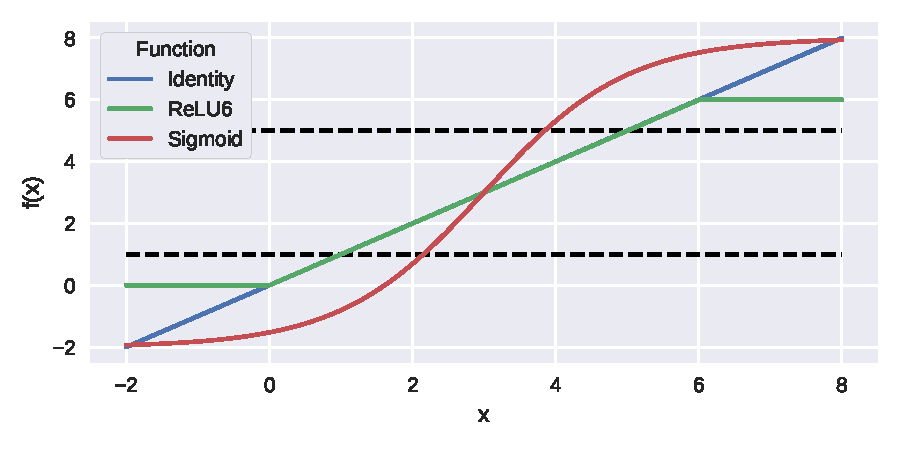
\includegraphics[width=0.8\linewidth]{functions_nn}
\caption{The three transformations considered at the output node for regression in a neural network. The dashed horizontal lines represent the boundary of observed ratings. }\label{fig:method.models.nn.functions}
\end{figure}

Fourth, we can treat our responses as five classes where only one is observed per example. In that case, we encode the ratings in the \textit{one-hot} fashion, that is, 4 gets encoded as $(0,0,0,1,0)$. Then, the final layer is transformed using the usual softmax function and the loss function used is the binary cross-entropy. Again, this encoding loses the ordinal nature of the ratings.

Fifth, we can choose a different encoding for the five classes that will reflect ordering of ratings. Indeed, we can encode a 4 as $(1,1,1,1,0)$ and model the responses in the multi-label classification way. Then, since all encoded responses have this ordinal structure, the NN will reproduce it in its predictions. In that case, we perform a sigmoid transformation on the five final nodes before comparing them to the encoded ratings; the loss function is again the binary cross-entropy.




\begin{figure}
\centering


\tikzset{every picture/.style={line width=0.75pt}} %set default line width to 0.75pt        

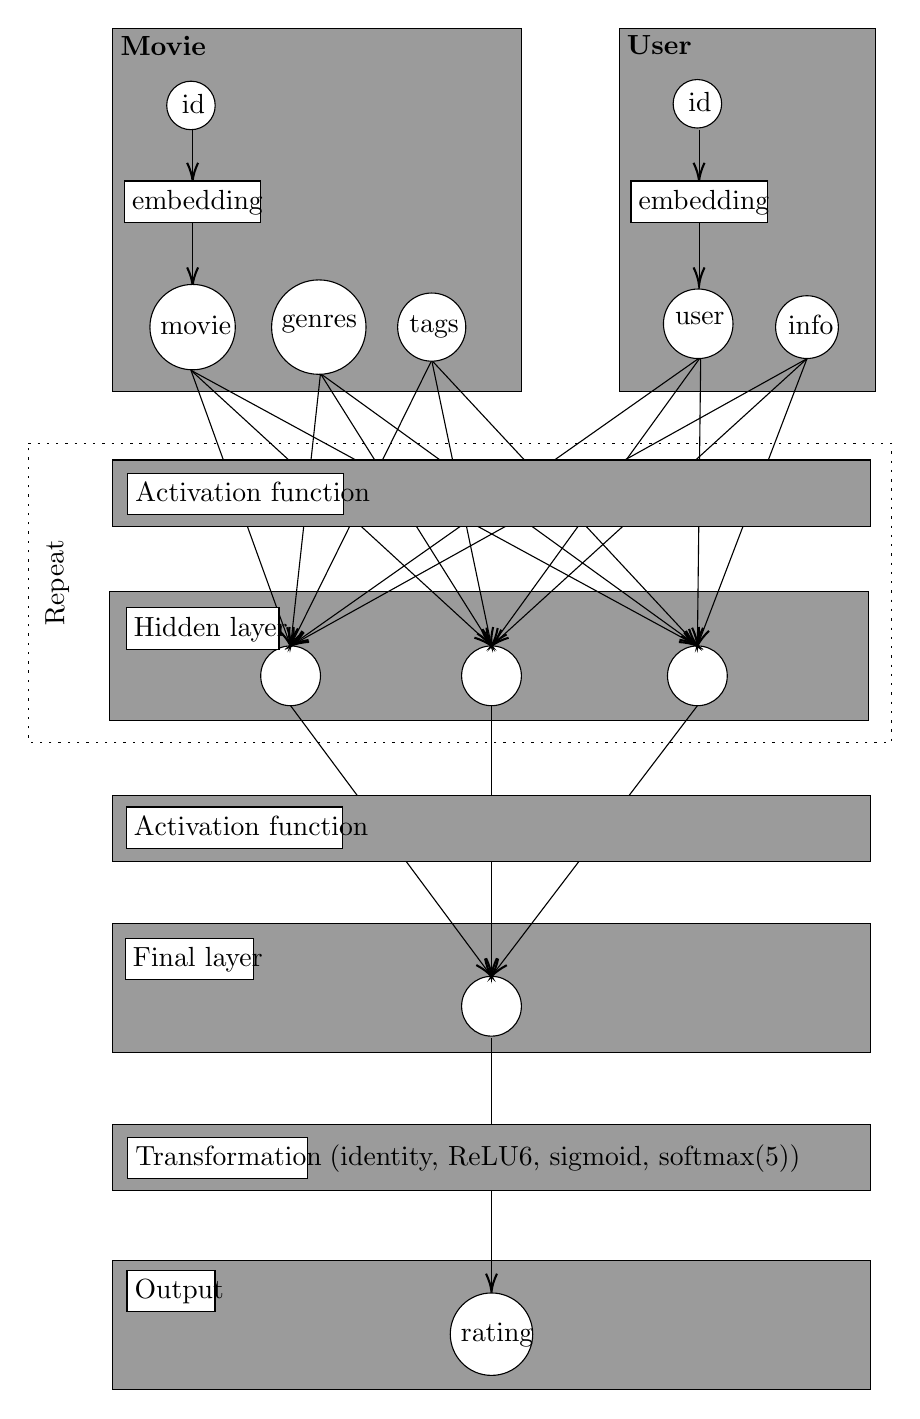
\begin{tikzpicture}[x=0.75pt,y=0.75pt,yscale=-1,xscale=1, scale=0.8]
%uncomment if require: \path (0,923); %set diagram left start at 0, and has height of 923

%Shape: Rectangle [id:dp2307314996446338] 
\draw  [fill={rgb, 255:red, 155; green, 155; blue, 155 }  ,fill opacity=1 ] (122,31) -- (368,31) -- (368,250) -- (122,250) -- cycle ;
%Straight Lines [id:da16141207798725943] 
\draw    (170,92) -- (170,121) ;
\draw [shift={(170,123)}, rotate = 270] [color={rgb, 255:red, 0; green, 0; blue, 0 }  ][line width=0.75]    (10.93,-3.29) .. controls (6.95,-1.4) and (3.31,-0.3) .. (0,0) .. controls (3.31,0.3) and (6.95,1.4) .. (10.93,3.29)   ;
%Straight Lines [id:da256251158457261] 
\draw    (170,148) -- (170,184) ;
\draw [shift={(170,186)}, rotate = 270] [color={rgb, 255:red, 0; green, 0; blue, 0 }  ][line width=0.75]    (10.93,-3.29) .. controls (6.95,-1.4) and (3.31,-0.3) .. (0,0) .. controls (3.31,0.3) and (6.95,1.4) .. (10.93,3.29)   ;
%Shape: Rectangle [id:dp4062601423389237] 
\draw  [fill={rgb, 255:red, 155; green, 155; blue, 155 }  ,fill opacity=1 ] (427,31) -- (581,31) -- (581,250) -- (427,250) -- cycle ;
%Straight Lines [id:da5944797488705584] 
\draw    (475,92) -- (475,121) ;
\draw [shift={(475,123)}, rotate = 270] [color={rgb, 255:red, 0; green, 0; blue, 0 }  ][line width=0.75]    (10.93,-3.29) .. controls (6.95,-1.4) and (3.31,-0.3) .. (0,0) .. controls (3.31,0.3) and (6.95,1.4) .. (10.93,3.29)   ;
%Straight Lines [id:da3036173249772247] 
\draw    (475,148) -- (475,184) ;
\draw [shift={(475,186)}, rotate = 270] [color={rgb, 255:red, 0; green, 0; blue, 0 }  ][line width=0.75]    (10.93,-3.29) .. controls (6.95,-1.4) and (3.31,-0.3) .. (0,0) .. controls (3.31,0.3) and (6.95,1.4) .. (10.93,3.29)   ;
%Shape: Rectangle [id:dp9997854452663028] 
\draw  [fill={rgb, 255:red, 155; green, 155; blue, 155 }  ,fill opacity=1 ] (120,370) -- (577,370) -- (577,448) -- (120,448) -- cycle ;
%Straight Lines [id:da5917985818254904] 
\draw    (169,237) -- (228.32,401.12) ;
\draw [shift={(229,403)}, rotate = 250.13] [color={rgb, 255:red, 0; green, 0; blue, 0 }  ][line width=0.75]    (10.93,-3.29) .. controls (6.95,-1.4) and (3.31,-0.3) .. (0,0) .. controls (3.31,0.3) and (6.95,1.4) .. (10.93,3.29)   ;
%Shape: Circle [id:dp6114587760100195] 
\draw  [fill={rgb, 255:red, 255; green, 255; blue, 255 }  ,fill opacity=1 ] (332,421) .. controls (332,411.06) and (340.06,403) .. (350,403) .. controls (359.94,403) and (368,411.06) .. (368,421) .. controls (368,430.94) and (359.94,439) .. (350,439) .. controls (340.06,439) and (332,430.94) .. (332,421) -- cycle ;
%Shape: Circle [id:dp553345531736126] 
\draw  [fill={rgb, 255:red, 255; green, 255; blue, 255 }  ,fill opacity=1 ] (456,421) .. controls (456,411.06) and (464.06,403) .. (474,403) .. controls (483.94,403) and (492,411.06) .. (492,421) .. controls (492,430.94) and (483.94,439) .. (474,439) .. controls (464.06,439) and (456,430.94) .. (456,421) -- cycle ;
%Shape: Circle [id:dp16008652747984975] 
\draw  [fill={rgb, 255:red, 255; green, 255; blue, 255 }  ,fill opacity=1 ] (211,421) .. controls (211,411.06) and (219.06,403) .. (229,403) .. controls (238.94,403) and (247,411.06) .. (247,421) .. controls (247,430.94) and (238.94,439) .. (229,439) .. controls (219.06,439) and (211,430.94) .. (211,421) -- cycle ;
%Straight Lines [id:da07936131606411578] 
\draw    (169,237) -- (472.24,402.04) ;
\draw [shift={(474,403)}, rotate = 208.56] [color={rgb, 255:red, 0; green, 0; blue, 0 }  ][line width=0.75]    (10.93,-3.29) .. controls (6.95,-1.4) and (3.31,-0.3) .. (0,0) .. controls (3.31,0.3) and (6.95,1.4) .. (10.93,3.29)   ;
%Straight Lines [id:da03140198678455175] 
\draw    (169,237) -- (348.53,401.65) ;
\draw [shift={(350,403)}, rotate = 222.52] [color={rgb, 255:red, 0; green, 0; blue, 0 }  ][line width=0.75]    (10.93,-3.29) .. controls (6.95,-1.4) and (3.31,-0.3) .. (0,0) .. controls (3.31,0.3) and (6.95,1.4) .. (10.93,3.29)   ;
%Straight Lines [id:da8972801381289985] 
\draw    (247,239) -- (229.22,401.01) ;
\draw [shift={(229,403)}, rotate = 276.26] [color={rgb, 255:red, 0; green, 0; blue, 0 }  ][line width=0.75]    (10.93,-3.29) .. controls (6.95,-1.4) and (3.31,-0.3) .. (0,0) .. controls (3.31,0.3) and (6.95,1.4) .. (10.93,3.29)   ;
%Straight Lines [id:da5048950093422406] 
\draw    (247,239) -- (472.38,401.83) ;
\draw [shift={(474,403)}, rotate = 215.85] [color={rgb, 255:red, 0; green, 0; blue, 0 }  ][line width=0.75]    (10.93,-3.29) .. controls (6.95,-1.4) and (3.31,-0.3) .. (0,0) .. controls (3.31,0.3) and (6.95,1.4) .. (10.93,3.29)   ;
%Straight Lines [id:da2676023756738023] 
\draw    (247,239) -- (348.94,401.31) ;
\draw [shift={(350,403)}, rotate = 237.87] [color={rgb, 255:red, 0; green, 0; blue, 0 }  ][line width=0.75]    (10.93,-3.29) .. controls (6.95,-1.4) and (3.31,-0.3) .. (0,0) .. controls (3.31,0.3) and (6.95,1.4) .. (10.93,3.29)   ;
%Straight Lines [id:da4547393022990093] 
\draw    (314,231) -- (229.89,401.21) ;
\draw [shift={(229,403)}, rotate = 296.3] [color={rgb, 255:red, 0; green, 0; blue, 0 }  ][line width=0.75]    (10.93,-3.29) .. controls (6.95,-1.4) and (3.31,-0.3) .. (0,0) .. controls (3.31,0.3) and (6.95,1.4) .. (10.93,3.29)   ;
%Straight Lines [id:da6479494477610002] 
\draw    (314,231) -- (472.64,401.54) ;
\draw [shift={(474,403)}, rotate = 227.07] [color={rgb, 255:red, 0; green, 0; blue, 0 }  ][line width=0.75]    (10.93,-3.29) .. controls (6.95,-1.4) and (3.31,-0.3) .. (0,0) .. controls (3.31,0.3) and (6.95,1.4) .. (10.93,3.29)   ;
%Straight Lines [id:da443095768705153] 
\draw    (314,231) -- (349.59,401.04) ;
\draw [shift={(350,403)}, rotate = 258.18] [color={rgb, 255:red, 0; green, 0; blue, 0 }  ][line width=0.75]    (10.93,-3.29) .. controls (6.95,-1.4) and (3.31,-0.3) .. (0,0) .. controls (3.31,0.3) and (6.95,1.4) .. (10.93,3.29)   ;
%Straight Lines [id:da35507587145535247] 
\draw    (476,229) -- (424.1,265.56) -- (230.64,401.85) ;
\draw [shift={(229,403)}, rotate = 324.84000000000003] [color={rgb, 255:red, 0; green, 0; blue, 0 }  ][line width=0.75]    (10.93,-3.29) .. controls (6.95,-1.4) and (3.31,-0.3) .. (0,0) .. controls (3.31,0.3) and (6.95,1.4) .. (10.93,3.29)   ;
%Straight Lines [id:da9486617458047818] 
\draw    (476,229) -- (474.02,401) ;
\draw [shift={(474,403)}, rotate = 270.65999999999997] [color={rgb, 255:red, 0; green, 0; blue, 0 }  ][line width=0.75]    (10.93,-3.29) .. controls (6.95,-1.4) and (3.31,-0.3) .. (0,0) .. controls (3.31,0.3) and (6.95,1.4) .. (10.93,3.29)   ;
%Straight Lines [id:da8058732839276246] 
\draw    (476,229) -- (351.17,401.38) ;
\draw [shift={(350,403)}, rotate = 305.90999999999997] [color={rgb, 255:red, 0; green, 0; blue, 0 }  ][line width=0.75]    (10.93,-3.29) .. controls (6.95,-1.4) and (3.31,-0.3) .. (0,0) .. controls (3.31,0.3) and (6.95,1.4) .. (10.93,3.29)   ;
%Straight Lines [id:da8260388432043336] 
\draw    (540,230) -- (230.75,402.03) ;
\draw [shift={(229,403)}, rotate = 330.90999999999997] [color={rgb, 255:red, 0; green, 0; blue, 0 }  ][line width=0.75]    (10.93,-3.29) .. controls (6.95,-1.4) and (3.31,-0.3) .. (0,0) .. controls (3.31,0.3) and (6.95,1.4) .. (10.93,3.29)   ;
%Straight Lines [id:da9400545257458622] 
\draw    (540,230) -- (474.71,401.13) ;
\draw [shift={(474,403)}, rotate = 290.88] [color={rgb, 255:red, 0; green, 0; blue, 0 }  ][line width=0.75]    (10.93,-3.29) .. controls (6.95,-1.4) and (3.31,-0.3) .. (0,0) .. controls (3.31,0.3) and (6.95,1.4) .. (10.93,3.29)   ;
%Straight Lines [id:da05542791968584537] 
\draw    (540,230) -- (351.48,401.65) ;
\draw [shift={(350,403)}, rotate = 317.68] [color={rgb, 255:red, 0; green, 0; blue, 0 }  ][line width=0.75]    (10.93,-3.29) .. controls (6.95,-1.4) and (3.31,-0.3) .. (0,0) .. controls (3.31,0.3) and (6.95,1.4) .. (10.93,3.29)   ;
%Shape: Rectangle [id:dp9672123809852601] 
\draw  [fill={rgb, 255:red, 155; green, 155; blue, 155 }  ,fill opacity=1 ] (121.5,291) -- (578.5,291) -- (578.5,331) -- (121.5,331) -- cycle ;
%Shape: Rectangle [id:dp27962627521584915] 
\draw  [dash pattern={on 0.84pt off 2.51pt}] (71,281) -- (591,281) -- (591,461) -- (71,461) -- cycle ;
%Shape: Rectangle [id:dp7643196245006507] 
\draw  [fill={rgb, 255:red, 155; green, 155; blue, 155 }  ,fill opacity=1 ] (121.5,570) -- (578.5,570) -- (578.5,648) -- (121.5,648) -- cycle ;
%Shape: Circle [id:dp2621970126778864] 
\draw  [fill={rgb, 255:red, 255; green, 255; blue, 255 }  ,fill opacity=1 ] (332,620) .. controls (332,610.06) and (340.06,602) .. (350,602) .. controls (359.94,602) and (368,610.06) .. (368,620) .. controls (368,629.94) and (359.94,638) .. (350,638) .. controls (340.06,638) and (332,629.94) .. (332,620) -- cycle ;
%Straight Lines [id:da7681063443100834] 
\draw    (229,439) -- (348.81,600.39) ;
\draw [shift={(350,602)}, rotate = 233.41] [color={rgb, 255:red, 0; green, 0; blue, 0 }  ][line width=0.75]    (10.93,-3.29) .. controls (6.95,-1.4) and (3.31,-0.3) .. (0,0) .. controls (3.31,0.3) and (6.95,1.4) .. (10.93,3.29)   ;
%Straight Lines [id:da5530075765034418] 
\draw    (350,439) -- (350,600) ;
\draw [shift={(350,602)}, rotate = 270] [color={rgb, 255:red, 0; green, 0; blue, 0 }  ][line width=0.75]    (10.93,-3.29) .. controls (6.95,-1.4) and (3.31,-0.3) .. (0,0) .. controls (3.31,0.3) and (6.95,1.4) .. (10.93,3.29)   ;
%Straight Lines [id:da8488306912122049] 
\draw    (474,439) -- (351.21,600.41) ;
\draw [shift={(350,602)}, rotate = 307.26] [color={rgb, 255:red, 0; green, 0; blue, 0 }  ][line width=0.75]    (10.93,-3.29) .. controls (6.95,-1.4) and (3.31,-0.3) .. (0,0) .. controls (3.31,0.3) and (6.95,1.4) .. (10.93,3.29)   ;
%Shape: Rectangle [id:dp9887981961930326] 
\draw  [fill={rgb, 255:red, 155; green, 155; blue, 155 }  ,fill opacity=1 ] (121.5,493) -- (578.5,493) -- (578.5,533) -- (121.5,533) -- cycle ;
%Shape: Rectangle [id:dp18515621761343992] 
\draw  [fill={rgb, 255:red, 155; green, 155; blue, 155 }  ,fill opacity=1 ] (121.5,773) -- (578.5,773) -- (578.5,851) -- (121.5,851) -- cycle ;
%Straight Lines [id:da2322651311514875] 
\draw    (350,639) -- (350,790) ;
\draw [shift={(350,792)}, rotate = 270] [color={rgb, 255:red, 0; green, 0; blue, 0 }  ][line width=0.75]    (10.93,-3.29) .. controls (6.95,-1.4) and (3.31,-0.3) .. (0,0) .. controls (3.31,0.3) and (6.95,1.4) .. (10.93,3.29)   ;
%Shape: Rectangle [id:dp7909457996411972] 
\draw  [fill={rgb, 255:red, 155; green, 155; blue, 155 }  ,fill opacity=1 ] (121.5,691) -- (578.5,691) -- (578.5,731) -- (121.5,731) -- cycle ;

% Text Node
\draw (125,34) node [anchor=north west][inner sep=0.75pt]   [align=left] {\textbf{Movie}};
% Text Node
\draw  [fill={rgb, 255:red, 255; green, 255; blue, 255 }  ,fill opacity=1 ]  (169, 77.5) circle [x radius= 14.6, y radius= 14.6]   ;
\draw (162,69) node [anchor=north west][inner sep=0.75pt]   [align=left] {id};
% Text Node
\draw  [fill={rgb, 255:red, 255; green, 255; blue, 255 }  ,fill opacity=1 ]  (246, 211) circle [x radius= 28.43, y radius= 28.43]   ;
\draw (222,202.5) node [anchor=north west][inner sep=0.75pt]   [align=left] {genres};
% Text Node
\draw  [fill={rgb, 255:red, 255; green, 255; blue, 255 }  ,fill opacity=1 ]  (314, 211) circle [x radius= 20.52, y radius= 20.52]   ;
\draw (299,202.5) node [anchor=north west][inner sep=0.75pt]   [align=left] {tags};
% Text Node
\draw  [fill={rgb, 255:red, 255; green, 255; blue, 255 }  ,fill opacity=1 ]  (129,123) -- (211,123) -- (211,148) -- (129,148) -- cycle  ;
\draw (132,127) node [anchor=north west][inner sep=0.75pt]   [align=left] {embedding};
% Text Node
\draw  [fill={rgb, 255:red, 255; green, 255; blue, 255 }  ,fill opacity=1 ]  (170, 211) circle [x radius= 25.71, y radius= 25.71]   ;
\draw (149,202.5) node [anchor=north west][inner sep=0.75pt]   [align=left] {movie};
% Text Node
\draw (430,34) node [anchor=north west][inner sep=0.75pt]   [align=left] {\textbf{User}};
% Text Node
\draw  [fill={rgb, 255:red, 255; green, 255; blue, 255 }  ,fill opacity=1 ]  (474, 76.5) circle [x radius= 14.6, y radius= 14.6]   ;
\draw (467,68) node [anchor=north west][inner sep=0.75pt]   [align=left] {id};
% Text Node
\draw  [fill={rgb, 255:red, 255; green, 255; blue, 255 }  ,fill opacity=1 ]  (540, 211) circle [x radius= 18.9, y radius= 18.9]   ;
\draw (527,202.5) node [anchor=north west][inner sep=0.75pt]   [align=left] {info};
% Text Node
\draw  [fill={rgb, 255:red, 255; green, 255; blue, 255 }  ,fill opacity=1 ]  (434,123) -- (516,123) -- (516,148) -- (434,148) -- cycle  ;
\draw (437,127) node [anchor=north west][inner sep=0.75pt]   [align=left] {embedding};
% Text Node
\draw  [fill={rgb, 255:red, 255; green, 255; blue, 255 }  ,fill opacity=1 ]  (474.5, 209) circle [x radius= 20.94, y radius= 20.94]   ;
\draw (459,200.5) node [anchor=north west][inner sep=0.75pt]   [align=left] {user};
% Text Node
\draw  [fill={rgb, 255:red, 255; green, 255; blue, 255 }  ,fill opacity=1 ]  (131,299) -- (261,299) -- (261,324) -- (131,324) -- cycle  ;
\draw (134,303) node [anchor=north west][inner sep=0.75pt]   [align=left] {Activation function};
% Text Node
\draw  [fill={rgb, 255:red, 255; green, 255; blue, 255 }  ,fill opacity=1 ]  (130,380) -- (222,380) -- (222,405) -- (130,405) -- cycle  ;
\draw (133,384) node [anchor=north west][inner sep=0.75pt]   [align=left] {Hidden layer};
% Text Node
\draw (79.86,392.62) node [anchor=north west][inner sep=0.75pt]  [rotate=-269.18] [align=left] {Repeat};
% Text Node
\draw  [fill={rgb, 255:red, 255; green, 255; blue, 255 }  ,fill opacity=1 ]  (130,500) -- (260,500) -- (260,525) -- (130,525) -- cycle  ;
\draw (133,504) node [anchor=north west][inner sep=0.75pt]   [align=left] {Activation function};
% Text Node
\draw  [fill={rgb, 255:red, 255; green, 255; blue, 255 }  ,fill opacity=1 ]  (129.5,579) -- (206.5,579) -- (206.5,604) -- (129.5,604) -- cycle  ;
\draw (132.5,583) node [anchor=north west][inner sep=0.75pt]   [align=left] {Final layer};
% Text Node
\draw  [fill={rgb, 255:red, 255; green, 255; blue, 255 }  ,fill opacity=1 ]  (131,699) -- (239,699) -- (239,724) -- (131,724) -- cycle  ;
\draw (134,703) node [anchor=north west][inner sep=0.75pt]   [align=left] {Transformation};
% Text Node
\draw  [fill={rgb, 255:red, 255; green, 255; blue, 255 }  ,fill opacity=1 ]  (130.5,779) -- (183.5,779) -- (183.5,804) -- (130.5,804) -- cycle  ;
\draw (133.5,783) node [anchor=north west][inner sep=0.75pt]   [align=left] {Output};
% Text Node
\draw  [fill={rgb, 255:red, 255; green, 255; blue, 255 }  ,fill opacity=1 ]  (350, 817.5) circle [x radius= 24.82, y radius= 24.82]   ;
\draw (330,809) node [anchor=north west][inner sep=0.75pt]   [align=left] {rating};
% Text Node
\draw (251,702) node [anchor=north west][inner sep=0.75pt]   [align=left] {(identity, ReLU6, sigmoid, softmax(5))};


\end{tikzpicture}

\caption{Neural network architecture described in \Cref{subsubsec:method.models.nn}. Black nodes represent observed quantities; white nodes, hidden variables; grey squares, functions.}
\label{fig:method.models.nn}
\end{figure}

%------------------------------------------------------------------------------
\paragraph{Implementation details.}\label{par:method.models.nn.impl}

Our NN models are implemented using the \texttt{PyTorch} module \citep{paszke2017automatic} using stochastic gradient descent. We use a fixed learning rate of \num{0.01}, batch size of \num{512} and number of epochs of \num{50}; the activation functions are chosen to be the ReLU function in all cases to reduce the tuning space. For this model, we have five tuning directions: movie and user embedding sizes, hidden layers number and sizes and the final transformation. We also compare whether including the external information improves on simply using the two embeddings.

%------------------------------------------------------------------------------
\subsubsection{Matrix completion}\label{subsubsec:method.models.svd}
Building a recommendation system by doing matrix completion is one of \textit{collaborative filtering} techniques. This means that we will try to suggest movies to an user by inspecting the ratings of ``similar'' users. To be more specific, it is assumed that the taste, or the ratings, made by users follows some low-rank structure, and use that assumption to make prediction. The idea of using SVD for movie recommendation is simple but it turns out to be successful in application. The winner in the Netflix prize competition used SVD as the main technique in their algorithm \citep{bennett2007netflix}. 

%------------------------------------------------------------------------------
\paragraph{Model description.}\label{par:method.models.svd.model}
In this model, we use 2 hyper-parameters, which are the embedding dimension $k$ and the number of iterations $I$. We set up and train the training data as follows.

\begin{enumerate}
\item Create a pivoted matrix $A$ in which rows are users and columns are movies. The $(i,j)$-cell of the matrix is the rating of user i for movie j, and is \texttt{NA} if there is no information about that in the training set. We also create a masked matrix which indicate which cell in pivot matrix is \texttt{NA}. After that, we fill the \texttt{NA} cells in $A$ with \texttt{0}.
\item Repeat $I$ times: 
\begin{itemize}
	\item Fill all the non-masked cell in $A$ with the original visible rating.
	\item Approximate $A$ by its truncated SVD of rank $k$. 
\end{itemize}
\end{enumerate}

By iterating two steps above, it allows us to reuse the visible information over and over, and extract the low rank structure of ratings. 


%------------------------------------------------------------------------------


%------------------------------------------------------------------------------
\paragraph{Implementation details.}\label{par:method.models.svd.impl}
We use the \texttt{svds} function from \texttt{scipy.sparse.linalg} module \citep{2020SciPy-NMeth} to compute truncated SVD of pivoted matrix and repeat the two steps above to get the reconstruction of users-movies ratings matrix. After that, the information from the reconstructed matrix is used as predictions. This model has two turning parameters: the dimension $k$ and number of iterations $I$.  


%------------------------------------------------------------------------------
\subsubsection{Restricted Boltzmann Machine}\label{subsubsec:method.models.rbm}
Similar to matrix completion, Restricted Boltzmann Machine (RBM) is also a collaborative filtering method. It assumes ratings of users are affected by some latent binary variables. We construct a probabilistic model where there is $F$ hidden nodes in total and a bipartite graph for each user connecting the hidden variables with the visible ratings. 

%------------------------------------------------------------------------------
\paragraph{Model description.}\label{par:method.models.rbm.model}

\begin{figure}
	\begin{table}
\centering
\caption{RBM result}
\label{tab:results.rbm}
\begin{tabular}{llllllll}
\toprule
     &     &      & \multicolumn{2}{c}{CV} & \multicolumn{2}{c}{Test}\\
     \cmidrule(lr){4-5}\cmidrule(lr){6-7}
Hidden nodes & Gibbs iterations  & learning rate &    MSE & Acc. & MSE & Acc.  \\
\midrule
15.0 & 5.0 & 1.0 &   1.0362 &      0.3609 &   1.0308 &        0.3682 \\
     & 1.0 & 1.0 &   1.0375 &      0.3607 &   1.0330 &        0.3682 \\
20.0 & 5.0 & 1.0 &   1.0375 &      0.3612 &   1.0320 &        0.3670 \\
25.0 & 5.0 & 1.0 &   1.0394 &      0.3603 &   1.0344 &        0.3669 \\
\bottomrule
\end{tabular}
\end{table}

	\caption{Restricted Boltzmann Machine in \Cref{subsubsec:method.models.rbm}. Each user has a graphical model connecting hidden variables and visible ratings. Weights $W_{ij}^{k}$ are shared among users.\label{fig:method.models.rbm}}
\end{figure}



Denote hidden variables by $\textbf{h} = (h_1, h_2,\dots, h_F)$ and suppose there are $K$ rating scores in total ($5$ for our data set). For now, to reduce the burden of notation, we only consider the model for each user and will talk about the connection between them later. For a given user, suppose $m$ movies were rated and write the visible ratings $\textbf{V} = (v_i^k)_{i,k}$ where $v_i^k = 1$ if movie $m$ was rated $k$ and $0$ otherwise. The generative model is defined by
\begin{equation}\label{GenModelRBM}
p(\textbf{V}, \textbf{h}) = \dfrac{1}{Z} \exp(-E(\textbf{V}, \textbf{h})),
\end{equation}
where $Z = \sum_{\textbf{V}', \textbf{h}'}$ is the normalization. The term $E(V, h)$ is so called \textit{energy} and defined by
\begin{equation}\label{EnergyRBM}
E(V,h) = - \sum_{i=1}^{m} \sum_{j=1}^{F} \sum_{k=1}^{K} W_{ij}^k h_j v_i^k - \sum_{i=1}^{m} \sum_{k=1}^{K} b_i^k v_i^k - \sum_{j=1}^{F} h_j b_j,
\end{equation}
where $W_{ij}^k$ is the weight connecting $h_j$ to $v_i^k$, $b_i^k$ is a bias term for $v_i^k$ and $b_j$ is the bias for $h_j$. Therefore, each user has a different bipartite graph model and visible ratings $\textbf{V}$, but they all share the same weight $(W_{ij}^k)$ and biases $(b_i^k), (b_j)$.   

From this, we can calculate the conditional probability 
\begin{equation}\label{pv|h}
p(v_i^k = 1| \textbf{h}) = \dfrac{\exp(b_{i}^{k} + \sum_{j=1}^{F} h_j W_{ij}^k)}{\sum_{l=1}^{k} \exp(b_{i}^{l} + \sum_{j=1}^{F} h_j W_{ij}^l)}, 
\end{equation}
and
\begin{equation}\label{ph|v}
p(h_j = 1 | \textbf{V}) = \sigma(b_j + \sum_{i=1}^{m}\sum_{k=1}^{K} v_i^k W_{ij}^{k}),
\end{equation}
where $\sigma$ is the sigmoid function. The marginal distribution for $\textbf{V}$ is
$$p(\textbf{V}) = \dfrac{1}{Z} \sum_{\textbf{h'}} \exp(-E(\textbf{V}, \textbf{h'})).$$
Our aim is to find $(W_{ij}^{k}, b_{i}^{k}, b_j)_{i,j,k}$ maximizing the marginal distribution for visible ratings $\textbf{V}$, which corresponds to the \textit{maximum likelihood} method. We will employ gradient descent to find the optimal weights. 

%------------------------------------------------------------------------------
\paragraph{Learning.}\label{par:method.models.rbm.learning}

We need to compute the gradient of $\log p(\textbf{V})$ in order to perform gradient ascent. By the chain rule
\begin{align*}
\dfrac{\partial \log p(\textbf{V})}{\partial W_{ij}^{k}} &= \dfrac{1}{p(\textbf{V})} \dfrac{\partial p(\textbf{V})}{\partial W_{ij}^{k}} \\
& = \dfrac{1}{p(\textbf{V})} \left(\dfrac{\sum_{\textbf{h}} \onebb_{[h_j = 1, v_{i}^{k} = 1]} p(\textbf{V}, \textbf{h})}{Z} - \dfrac{p(\textbf{V}) \sum_{\boldsymbol{\nu}, \textbf{h}}\onebb_{[h_j = 1, \boldsymbol{\nu}_{i}^{k} = 1]} p(\boldsymbol{\nu}, \textbf{h})}{Z} \right)\\
& = \Ebb_{h|\textbf{V}}(v_i^k h_j) - \Ebb(\nu_i^k h_j)\\
& =: \cexp{v_i^k h_j}_{data} - \cexp{\nu_i^k h_j}_{model}
\end{align*}
where $\cexp{\cdot}_{subscript}$ denotes the conditional expectation with respect to the subscript. 
Similarly, we have
\begin{equation}
\dfrac{\partial p(\textbf{V})}{\partial b_j}  = \Ebb_{h|\textbf{V}} (h_j) - \Ebb(h_j) =  \cexp{h_j}_{data} - \cexp{h_j}_{model},
\end{equation}
and 
\begin{equation}
\dfrac{\partial p(\textbf{V})}{\partial b_i^k}  = v_i^k - \Ebb(\nu_i^k) = v_i^k - \cexp{\nu_i^k}_{model}.
\end{equation}
In each equation, it is customary to call the first term \textit{positive statistics} and second term \textit{negative statistics}. Hence, we have the analytical representation of gradient of weights and biased terms. In every equation, the first term is easy to compute thanks to \eqref{ph|v}. However, computing the terms $\cexp{\nu_{i}^{k}}_{model}, \cexp{h_j}_{model}$, and $\cexp{\nu_{i}^{k}}_{model}$ requires to take the sum over all value of $\boldsymbol{\nu}, \textbf{h}$, which takes exponential time and makes the algorithm inefficiently. We will instead use the \textit{Contrastive Divergence} (CD) method \citep{hinton2012practical} which consists of approximating $\cexp{\nu_i^k h_j}_{model}$ with $\cexp{\nu_i^k h_j}_{recon}$, an approximated reconstruction of $\cexp{\nu_i^k h_j}_{model}$ based on an idea similar to the Gibbs' sampler.

%------------------------------------------------------------------------------
\paragraph{Computing gradient using Constrastive Divergence.}\label{par:method.models.rbm.grad}

The idea behind Contrastive Divergence \citep{hinton2012practical} is to approximate the gradient using the difference of two Kullback-Leibler divergences and ignore one trickly term. Although this is a crude approximation, it turns out to work really well in many applications. The Constrastive Divergence with $n$ steps ($CD_n$) can be interpreted as follows. Given the visible ratings $\textbf{V}$, first we sample binary value for hidden units $h_{data} = h$ by equation \eqref{ph|v}. Then we do $n$ steps of Gibbs' sampling, each contains two intermediary steps
\begin{enumerate}
	\item Sample $\boldsymbol{\nu} \leftarrow \boldsymbol{h}$ based on equation \eqref{pv|h}.
	\item Sample $\boldsymbol{h} \leftarrow \boldsymbol{\nu}$ based on equation \eqref{ph|v}.
\end{enumerate}
To derive the positive statistics, we use the value of data $\textbf{V}$ and $h_{data}$. Although we can calculate it analytically using \eqref{ph|v}, using the sample values can reduce the noise when we take the difference with the negative statistics. Hence, we have
$$\cexp{v_i^k h_j}_{data} \leftarrow v_i^k h_{data, j}, \quad \cexp{h_j}_{data} \leftarrow h_{data, j}$$
When collect the negative statistics, it is advised in \cite{hinton2012practical} that in the last step, we should only collect $\boldsymbol{h}$ as the probability $p(\textbf{h}|\boldsymbol{\nu})$ (but not sample from it) to get the updates
$$\cexp{\nu_i^k h_j}_{recon} \leftarrow \nu_i^k h_{j},\quad \cexp{h_j}_{recon} \leftarrow h_{data, j},\quad \cexp{\nu_i^k}_{recon} \leftarrow \nu_i^k.$$

%------------------------------------------------------------------------------
\paragraph{Making predictions.}\label{par:method.models.rbm.pred}

Given a set of visible unit $\textbf{V}$, we can predict the rating for a new movie by using Bayes' rule and marginalization of $\textbf{h}$:
\begin{align*}
p(v_q^{k} =  1 |\textbf{V}) & \propto p(v_q^{k} = 1, \textbf{V})  \\
&  \propto \sum_{\textbf{h}} p(v_q^{k} = 1, \textbf{V}, \textbf{h})\\
& \propto \exp(b_k^q) \prod_{j=1}^{q} \sum_{h_j\in \{0,1\}} \exp(\sum_{il} v_i^{l} h_j W_{ij}^{l} + h_j W_{qj}^{k} + h_jb_j)\\
& = \exp(b_k^q) \prod_{j=1}^{q} \left( 1 +  \exp(\sum_{il} v_i^{l} W_{ij}^{l} +  W_{qj}^{k} + b_j)\right)
\end{align*}


%------------------------------------------------------------------------------
\paragraph{Implementation details.}\label{par:method.models.rbm.impl}

We build and train a RBM model by ourselves using basic modules such as \texttt{numpy} \citep{numpy2011}. There are three turning parameters in the model: the number of hidden nodes, the number of Gibbs samplings in Contrastive Divergence, and the learning rate. Many details in the implementation are taken from \cite{hinton2012practical}.


%------------------------------------------------------------------------------
\section{Results}\label{sec:results}

We perform 5-fold cross-validation on many instances of our models against the training set and produce the \textit{mean squared error} (MSE) and prediction accuracy averaged over the 5 folds. For models with numerical predictions, we assign the predicted rating to the nearest integer in the range $[1,5]$.  Models with class predictions simply use the class label as their numerical prediction. 

It is worthwhile to mention that we are in a classification problem with 5 classes so a random assignment would produce 20\% accuracy: we observe accuracies close to 40\%, which is already a great improvement. MSEs less than 1 means that the model predicts, on average, ratings less than 1 point away from the recorded ratings.

We first detail the results for the four models we consider, noting some observation on their CV performance. Then, we proceed to a comparison of the four models in terms of CV and testing.

%------------------------------------------------------------------------------
\subsection{$K$-Nearest-Neighbors}\label{sebsec:results.knn}

Upon training and testing 35 instances of the $K$-NN model described in \Cref{subsubsec:method.models.knn} with varying tuning parameters, we obtain the results depicted in \Cref{tab:results.knn} which contains a selection of the best models.

As could be expected, regression aggregation performs better in terms of MSE while classification aggregation performs better in terms of prediction accuracy. Also, the value of the tuning parameters $\alpha_\text{user}$ and $\alpha_\text{tags}$ for these best models seems to align with their purpose. Indeed, we observe that the best models require to inflate the importance of user information and deflate that of tags.

The  $K$-NN models is particularly inefficient computationally: when $K$ increases from 5 to 100, training time increases from minutes to hours.

\begin{table}
\centering
\begin{tabular}{lrrrrrrr}
\toprule
           &     & \multicolumn{2}{c}{$\alpha$} &  \multicolumn{2}{c}{CV} & \multicolumn{2}{c}{Test} \\
           \cmidrule(lr){3-4}\cmidrule(lr){5-6}\cmidrule(l){7-8}
Aggregation & $K$ & User & Tags &  MSE & Acc. & MSE & Acc.  \\
\midrule
Regressor & 50  & 200  & 0.5 &  0.9898 &      0.3741 &   0.9737 &        0.3767 \\
           &     & 1000 & 1.0 &  0.9950 &      0.3733 &   0.9780 &        0.3779 \\
           &     & 500  & 0.5 &  0.9966 &      0.3725 &   0.9802 &        0.3762 \\
           &     & 200  & 0.2 &  1.0129 &      0.3703 &   0.9967 &        0.3742 \\
           &     & 500  & 0.2 &  1.0129 &      0.3702 &   0.9967 &        0.3742 \\
           & 75  & 200  & 0.5 &  1.0145 &      0.3680 &   0.9972 &        0.3714 \\
           & 100 & 100  & 1.0 &  1.0166 &      0.3690 &   1.0045 &        0.3694 \\
Classifier & 100 & 100  & 1.0 &  1.2363 &      0.3900 &   1.2395 &        0.3915 \\
           & 50  & 100  & 1.0 &  1.2482 &      0.3935 &   1.2547 &        0.3940 \\
           & 100 & 1000 & 1.0 &  1.2979 &      0.3885 &   1.2759 &        0.3943 \\
           &     & 100  & 0.1 &  1.3521 &      0.3832 &   1.3454 &        0.3832 \\
           &     & 1000 & 0.1 &  1.3533 &      0.3833 &   1.3484 &        0.3831 \\
\bottomrule
\end{tabular}
\caption{sdfsdfs}
\label{tab:results.knn}
\end{table}



%------------------------------------------------------------------------------
\subsection{Neural Network}\label{sebsec:results.nn}

We trained over 400 instances of the NN approach described in \Cref{subsubsec:method.models.nn}; the results for a selection of the best models can be found in \Cref{tab:results.nn}. We make some observations with regards to the tuning parameters.

First, we observe that including the external features (genre, tags, user info) greatly improves the model as we see a 8\% relative reduction in the respective best MSE and a 5\% relative increase in the best respective accuracy. 

Second, we note that the ordinal transformation does not appear in the best results: inspecting the complete logs, we find that this method performs better than classification in terms of MSE but worse in terms of prediction and is therefore in the middle of the pack in both categories. The classification scheme yields good prediction performance, but we see accuracies similar to those from regression approaches. The three regression transformation---identity, ReLU6 and sigmoid---seem to perform rather similarly with the sigmoid transform being slightly worse generally.

Third, the best performing models in terms of CV metrics seem to require simpler hidden layers structures: while the experiments included networks with up to four hidden layers, the best models generally contain only two. This exhibits the benefit of using CV for model selection as it prevents overfitting.

In terms of computing time, the NN models we consider train for 50 epochs in around 1 minute on GPU.


\begin{table}
\centering
\begin{tabular}{lrr>{\raggedright\arraybackslash}p{3.6cm}cccc}
\toprule
           & \multicolumn{2}{c}{Embeddings} &     &  \multicolumn{2}{c}{CV} & \multicolumn{2}{c}{Test} \\
           \cmidrule(lr){2-3}\cmidrule(lr){5-6}\cmidrule(l){7-8}
Transform & User & Movie & Hidden layers &  MSE & Acc. & MSE & Acc.  \\
\midrule
\multicolumn{8}{c}{\textbf{With features}}\\\addlinespace
ReLU6 & 64 & 128 & (1024,~ReLU), (64,~ReLU) &  0.9855 &      0.3851 &   0.9552 &        0.3823 \\
Identity & 64 & 128 & (1024,~ReLU), (128,~ReLU) &  0.9857 &      0.3778 &   0.9360 &        0.4006 \\
Sigmoid & 32 & 64  & (1024,~ReLU), (256,~ReLU), (64,~ReLU) &  0.9953 &      0.3803 &   0.9439 &        0.3946 \\
ReLU6 & 32 & 128 & (1024,~ReLU), (256,~ReLU), (64,~ReLU) &  1.0124 &      0.3735 &   0.9853 &        0.3882 \\
           & 64 & 128 & (1024,~ReLU), (256,~ReLU), (64,~ReLU) &  1.0137 &      0.3826 &   0.9318 &        0.3974 \\
           & 32 & 64  & (1024,~ReLU), (128,~ReLU) &  1.0149 &      0.3709 &   1.0081 &        0.3653 \\
           &    &     & (1024,~ReLU), (64,~ReLU) &  1.0162 &      0.3674 &   1.0216 &        0.3614 \\
           &    & 128 & (512,~ReLU), (64,~ReLU) &  1.0168 &      0.3695 &   1.0101 &        0.3683 \\
Identity & 32 & 64  & (512,~ReLU), (64,~ReLU) &  1.0182 &      0.3665 &   1.0352 &        0.3563 \\
ReLU6 & 32 & 128 & (1024,~ReLU), (128,~ReLU) &  1.0183 &      0.3694 &   0.9866 &        0.3775 \\
           & 64 & 128 & (512,~ReLU), (64,~ReLU) &  1.0198 &      0.3696 &   0.9878 &        0.3692 \\
Sigmoid & 64 & 128 & (512,~ReLU), (64,~ReLU) &  1.0482 &      0.3865 &   1.0510 &        0.3964 \\
Classifier & 64 & 64  & (1024,~ReLU), (64,~ReLU) &  1.1232 &      0.3780 &   1.1096 &        0.3864 \\
           &    &     & (1024,~ReLU), (128,~ReLU) &  1.1239 &      0.3786 &   1.1156 &        0.3845 \\
           &    & 128 & (1024,~ReLU), (64,~ReLU) &  1.1298 &      0.3786 &   1.1110 &        0.3899 \\
           \midrule
\multicolumn{8}{c}{\textbf{Without features}}\\\addlinespace
ReLU6 & 32  & 128 & (512,~ReLU), (64,~ReLU) &  1.0633 &      0.3620 &   1.0480 &        0.3677 \\
Identity & 32  & 128 & (512,~ReLU), (128,~ReLU) &  1.0652 &      0.3576 &   1.0500 &        0.3639 \\
ReLU6 & 32  & 128 & (512,~ReLU), (128,~ReLU) &  1.0732 &      0.3621 &   1.0738 &        0.3575 \\
                 & 64  & 128 & (128,~ReLU), (64,~ReLU), (64,~ReLU) &  1.0741 &      0.3585 &   1.0976 &        0.3487 \\
Identity & 64  & 128 & (1024,~ReLU), (128,~ReLU) &  1.0768 &      0.3589 &   1.0982 &        0.3525 \\
ReLU6 & 32  & 128 & (1024,~ReLU), (64,~ReLU) &  1.0768 &      0.3617 &   1.0469 &        0.3672 \\
                 & 64  & 128 & (1024,~ReLU), (64,~ReLU) &  1.0775 &      0.3604 &   1.0830 &        0.3584 \\
                 & 32  & 128 & (256,~ReLU), (128,~ReLU) &  1.0797 &      0.3614 &   1.0701 &        0.3531 \\

\bottomrule
\end{tabular}
\caption{Cross-validation and testing metrics of some of the best neural network models trained on the \texttt{MovieLens} dataset. The complete logs can be found alongside the project's code at \url{https://github.com/fontaine618/507-Project/}.}
\label{tab:results.nn}
\end{table}



%------------------------------------------------------------------------------
\subsection{Matrix completion}\label{sebsec:results.svd}
We trained around 100 instances of matrix completion models described in \Cref{subsubsec:method.models.svd}. We choose to present some models with its parameters. From the result, in \Cref{tab:results.svd}, we can see some facts about turning parameters as below.

For the embedded dimension $k$, if it is chosen to be too small, the model will not capture enough the complexity of the data and lead to the underfitting phenomena. If $k$ is large, the computational time will relatively increase but the prediction is not getting better, and there is even the overfitting phenomena. 

For the iterative number $I$ to use SVD, it can be seen that small $I$ leads to underfitting model meanwhile large $I$ leads to overfitting model. This can be interpreted that if we reuse the training data too many times, the model will tend to prefer the training data and the test error will eventually increase. If $k$ and $I$ are large at the same time, the model will be surely overfitting.

It is amazing that this model only needs a few lines of code but the performance is comparable to what the complicated models like Neural network or Restricted Boltzmann Machine do. The idea behind this method is also innocent and it is computationally efficient (most of them only take less than a second to train in a 4 cores CPU machine).     

\begin{table}
\centering
\caption{SVD result}
\label{tab:results.svd}
\begin{tabular}{llllll}
\toprule
  &     &   \multicolumn{2}{c}{CV} & \multicolumn{2}{c}{Test}\\
  \cmidrule(lr){3-4}\cmidrule(lr){5-6}
Dimension & Iteration numbers &        MSE & Acc. & MSE & Acc.  \\
\midrule
4 & 100 &  0.9533 &      0.4116 &   0.8810 &        0.4333 \\
5 & 100 &  0.9774 &      0.4103 &   0.9038 &        0.4306 \\
4 & 80  &  0.9804 &      0.4081 &   0.8954 &        0.4298 \\
  & 70  &  1.0014 &      0.4046 &   0.9075 &        0.4271 \\
5 & 80  &  1.0024 &      0.4049 &   0.9206 &        0.4257 \\
  & 70  &  1.0220 &      0.4016 &   0.9338 &        0.4236 \\
\bottomrule
\end{tabular}
\end{table}


%------------------------------------------------------------------------------
\subsection{Restricted Bolztmann Machine}\label{sebsec:results.rbm}

We trained around 100 instances of RBM model as describes in \Cref{subsubsec:method.models.rbm}. We choose to present some models with its parameters. From the result, in \Cref{tab:results.rbm}, we can see some facts about turning parameters as below.

For the number of hidden nodes, it turns out to be the best when set it around 15-20. If this number is too small, the model will be underfitting, but setting this number to large does not help the model to predict better.

For the number of Gibbs samplings to use in Contrastive Divergence, it is plausible to set it 1, because it does not help to improve the model significantly when it increases, but slow down the learning phase much (we need to do sampling for every (movie, user) couple.)

It is claimed in \cite{10.1145/1273496.1273596} that RBM paper can outperform SVD models in a fine-tuned parameters scenario. However, we observe something contrary to that here. It may due to the fact that the research team at the University of Toronto spent several years to achieve the expertise in training RBM models. In the time to the final report, we will keep trying improve our RBM model and see how far can we go compared to which is presented in that paper.

\begin{table}
\centering
\caption{RBM result}
\label{tab:results.rbm}
\begin{tabular}{llllllll}
\toprule
     &     &      & \multicolumn{2}{c}{CV} & \multicolumn{2}{c}{Test}\\
     \cmidrule(lr){4-5}\cmidrule(lr){6-7}
Hidden nodes & Gibbs iterations  & learning rate &    MSE & Acc. & MSE & Acc.  \\
\midrule
15.0 & 5.0 & 1.0 &   1.0362 &      0.3609 &   1.0308 &        0.3682 \\
     & 1.0 & 1.0 &   1.0375 &      0.3607 &   1.0330 &        0.3682 \\
20.0 & 5.0 & 1.0 &   1.0375 &      0.3612 &   1.0320 &        0.3670 \\
25.0 & 5.0 & 1.0 &   1.0394 &      0.3603 &   1.0344 &        0.3669 \\
\bottomrule
\end{tabular}
\end{table}


%------------------------------------------------------------------------------
\subsection{Model comparison}\label{sebsec:results.model}

\Cref{tab:results.model} contains a comparison of the best version of each of the four models we consider in terms of both regression and classification metrics. Overall, matrix completion using SVD systematically out-performs all other models in MSE and classification accuracy.

The $K$-NN models perform worse than $NN$ and matrix completion and require much more computing time. This approach does not seem very promising as a predictive model for movie ratings.

The $NN$ models yield interesting results and can be trained efficiently, but they do not achieve the performance level of matrix completion even though more information is included in the model. Indeed, matrix completion does not use movie genre and tags nor user details.

The SVD matrix completion model, it can be seen that this simple model can outperform many other complicated models. Simon Funk, a participant in the Netflix prize competition \citep{bennett2007netflix}, used this simple model and finished in third place.\footnote{\url{https://sifter.org/~simon/journal/20061211.html}} Its computational efficiency, compared to all three other models, is also a very appealing feature.

The RBM model, while a beautiful latent variable model, really needs time and expertise to be able to set it up correctly and implemenent efficiently.  

\begin{table}
\centering
\caption{sdfsdfs}
\label{tab:results.model}
\begin{tabular}{lrrrr}
\toprule
	      &  \multicolumn{2}{c}{CV} & \multicolumn{2}{c}{Test} \\
           \cmidrule(lr){2-3}\cmidrule(lr){4-5}
Model	 &  MSE & Acc. & MSE & Acc.  \\
\midrule
\multicolumn{5}{c}{\textbf{Best regressor}}\\
$K$-Nearest-Neighbors 					&   0.9898 &      0.3741 &   0.9737 &        0.3767 \\
Neural Network 							&   0.9855 &      0.3851 &   0.9552 &        0.3823 \\
Matrix completion 						&   0.9533 &      0.4116 &   0.8810 &        0.4333 \\
Restricted Boltzmann Machine 			&   1.0362 &      0.3609 &   1.0308 &        0.3682 \\
\midrule
\multicolumn{5}{c}{\textbf{Best classifier}}\\
$K$-Nearest-Neighbors 					&   1.2482 &      0.3935 &   1.2547 &        0.3940 \\
Neural Network 							&   1.0482 &      0.3865 &   1.0510 &        0.3964 \\
Matrix completion 						&   1.0360 &      0.4116 &   0.9632 &        0.4333 \\
Restricted Boltzmann Machine 			&   1.1115 &      0.3609 &   1.1033 &        0.3682 \\
\bottomrule
\end{tabular}
\end{table}


%------------------------------------------------------------------------------
\section{Final report}\label{sec:final}

For the final report, we will use results from the above model comparison in order to select a final model. Then, we will proceed to an exploratory data analysis using that model in order to extract insight about ratings with respect to user and movie information.

%------------------------------------------------------------------------------
\newpage
\bibliographystyle{imsart-nameyear}
\bibliography{../utils/references}{}





\end{document}
